\subsubsection{Placement des collisions}
Une fois que le modèle est affiché et que tous les obstacles et éléments de
décors sont placés, il faut qu'on puisse intéragir avec eux.
\\ \\
Pour éviter de passer à travers les murs il faut detecter quand le joueur
est à la même position que le mur en question.
\\ \\
On a choisi d'abord d'afficher le modèle 3D, ensuite grâce à l'éditeur on
place des "boites" de collisions. En jeu ces boîte seront invisible, mais
infranchissable, ça permet de ne pas traverser les obstacles.
\\ \\
Par exemple on modelise une table avec le moteur 3D. Dans l'éditeur on rajoute
manuellement une "boite" de collisions à l'emplacement de la table, on cherche
à épouser la forme de la table. En jeu on verra que la table, et on ne pourra
pas la traverser, on peut même monter dessus etc.
\\ \\
Sur la figure \ref{fig:fig2} montre les différents types de "boîtes" On voit qu'on dessine
chaque éléments avec des boîtes.



\begin{figure}[H]
    \centering
    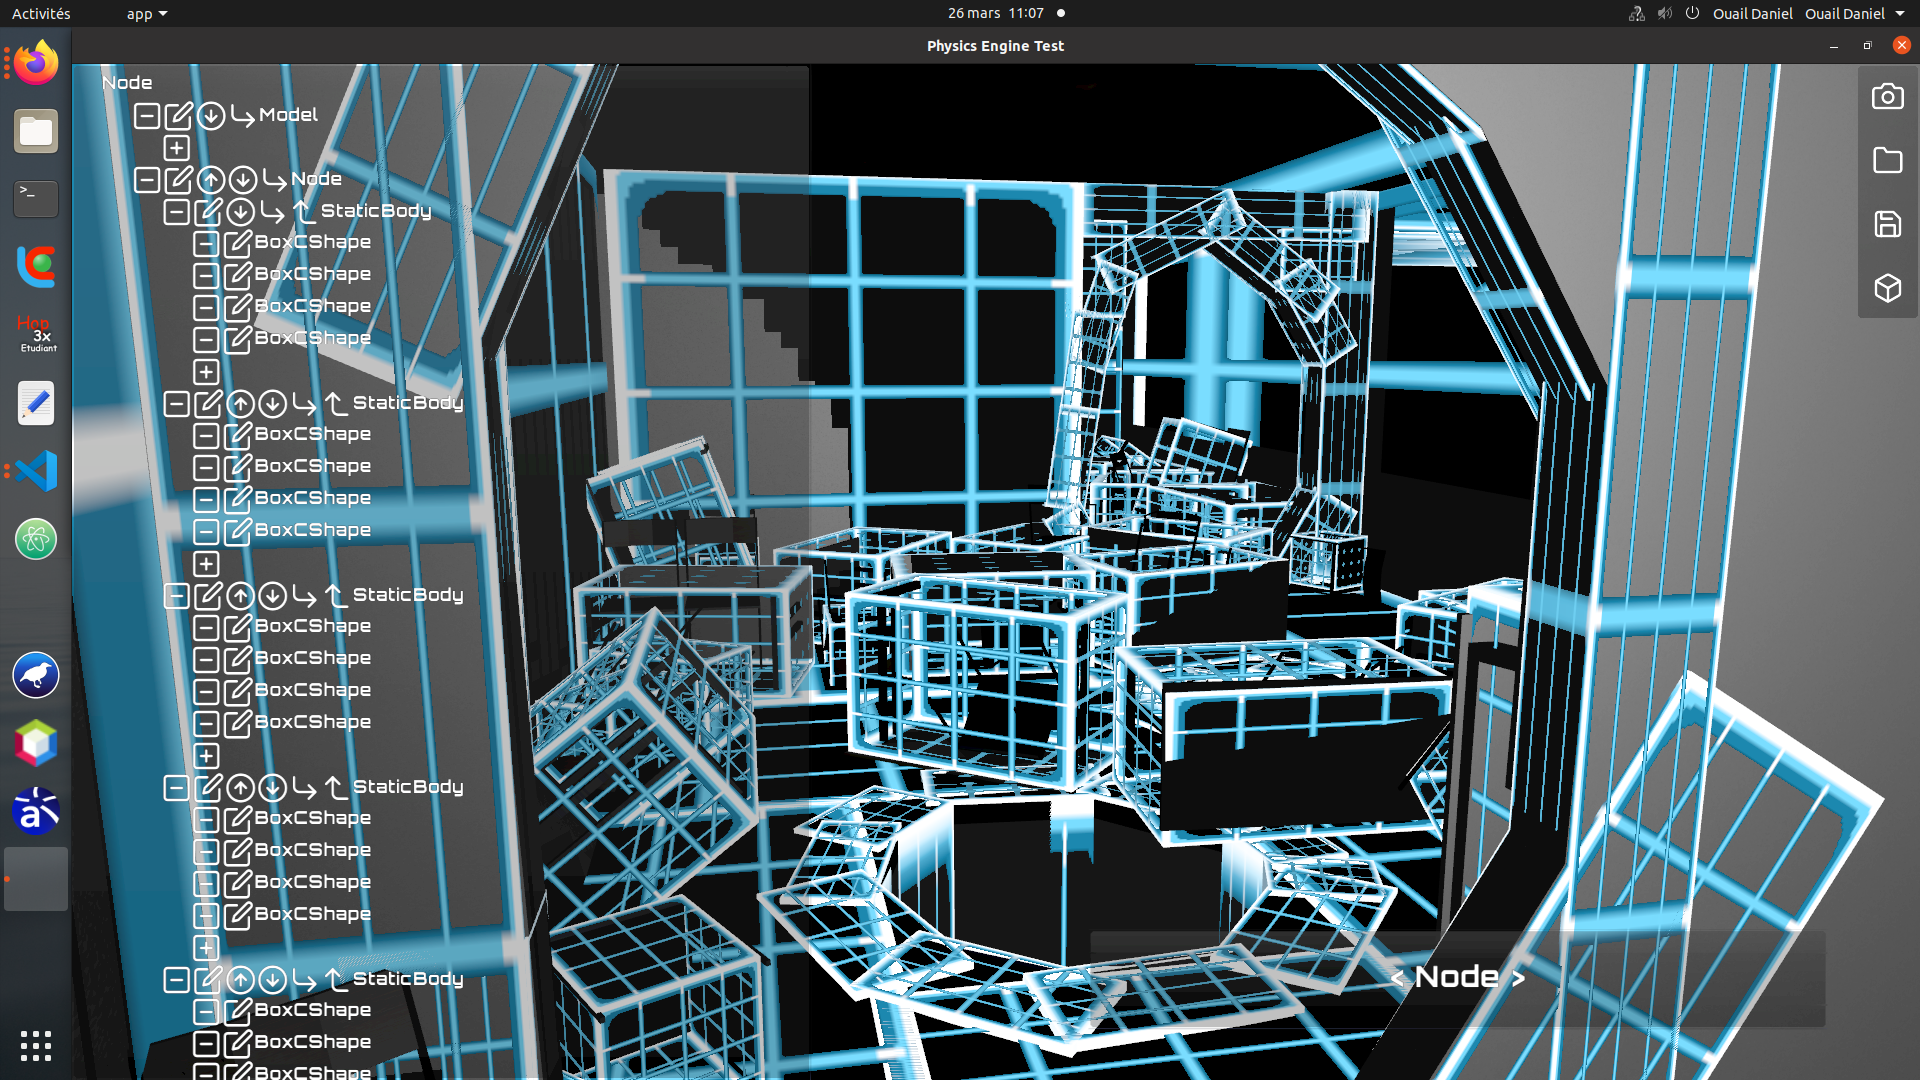
\includegraphics[width=1\linewidth]{images/screenshot_editeur.png}
    \caption{Capture d'écran de l'éditeur de niveau}
    \label{fig:fig2}
\end{figure}

Les coordonnées de chaque boîtes de collisions sont enregistrées avec l'éditeur
dans un fichier .scene, ce fichier sera lu au moment de l'execution pour
charger le modèle et les collisions.



\newpage